\documentclass[conference]{IEEEtran}

\usepackage[utf8]{inputenc}
\usepackage{amsmath}
\usepackage{graphicx}
\usepackage[table]{xcolor}
\usepackage{multirow}
\usepackage{colortbl}
\usepackage{hyperref}   % Para usar hipervínculos
\hypersetup{
    colorlinks=true,
    linkcolor=blue,
    filecolor=magenta,      
    urlcolor=cyan,
}

% --- TÍTULO Y AUTORES ---
\title{Integración de Tablas, Figuras y Bibliografía en IEEEtran}

\author{
    \IEEEauthorblockN{Autor Uno}
    \IEEEauthorblockA{
        Facultad de Ingeniería\\
        Universidad Ejemplo\\
        Ciudad, País\\
        \texttt{autor1@ejemplo.com}
    }
    \and
    \IEEEauthorblockN{Autor Dos}
    \IEEEauthorblockA{
        Departamento de Ciencias\\
        Otra Universidad\\
        Ciudad, País\\
        \texttt{autor2@ejemplo.com}
    }
}

\begin{document}

\maketitle

\begin{abstract}
    Este documento, preparado para el curso de Metodología de la Investigación, demuestra la correcta inserción de elementos complejos como tablas multicolumna, figuras con descripción y un sistema de referencias bibliográficas utilizando BibTeX en la plantilla IEEEtran.
\end{abstract}

\begin{IEEEkeywords}
IEEE, LaTeX, tabla, figura, bibliografía, BibTeX.
\end{IEEEkeywords}


\section{Introducción}
Este documento sigue la plantilla \texttt{IEEEtran} para artículos de conferencia. La gestión de referencias es crucial para la escritura académica, permitiendo dar crédito a trabajos previos y fundamentar la investigación actual. El desarrollo de redes neuronales ha sido un área de gran interés en los últimos años, como se discute en \cite{wu2018development}.


\section{Desarrollo del Contenido}
A continuación, se presentan los elementos solicitados integrados en el cuerpo del artículo.

\subsection{Tabla de Resultados}
Las tablas son una forma eficiente de presentar datos comparativos. La Tabla \ref{tab:resultados_exp} muestra un ejemplo que combina celdas para agrupar información relevante.

% --- TABLA ---
\begin{table}[h!]
\caption{Resultados Comparativos de Algoritmos}
\label{tab:resultados_exp}
\centering
\definecolor{lightgray}{gray}{0.9}
\rowcolors{2}{}{lightgray} 
\begin{tabular}{|c|l|c|c|}
\hline
\rowcolor{gray!40}
\multirow{2}{*}{\textbf{ID}} & \multicolumn{2}{c|}{\textbf{Métricas de Rendimiento}} & \multirow{2}{*}{\textbf{Observación}} \\ \cline{2-3}
\rowcolor{gray!40}
& \textbf{Precisión (\%)} & \textbf{Tiempo (s)} & \\ \hline
Algoritmo A & 92.5 & 1.23 & Normal \\ \hline
Algoritmo B & 95.1 & 2.45 & Lento \\ \hline
Algoritmo C & 94.8 & 0.89 & \textbf{Óptimo} \\ \hline
\end{tabular}
\end{table}

\subsection{Análisis Visual}
Las figuras son indispensables para mostrar tendencias. La Figura \ref{fig:diagrama_bloques} ilustra un diagrama de bloques. La aplicación de la inteligencia artificial en campos como la medicina ha revolucionado los diagnósticos y tratamientos \cite{hamet2017artificial}.

\begin{figure}[h!]
\centering
% Recuerda poner tu imagen (ej. mi_diagrama.png) en la misma carpeta
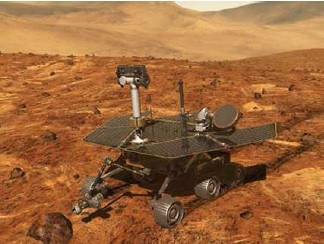
\includegraphics[width=0.9\columnwidth]{ejemplo.jpg}
\caption{Imagen de robot en la superficie terrestre de Marte.}
\label{fig:diagrama_bloques}
\end{figure}


\section{Conclusión}
Se han integrado exitosamente una tabla compleja, una figura descriptiva y un sistema de referencias bibliográficas en la plantilla \texttt{IEEEtran}, cumpliendo con los requisitos de la tarea.

\bibliographystyle{IEEEtran} 

% Llama al archivo .bib para generar la lista de referencias aquí
\bibliography{bibliografia}


\end{document}